%% fig06-flat-gather, caption is in docs/figures/README.md
\documentclass[border=8pt]{standalone}
% Shared preamble for the interpolation-geometry figures.
% \input by every figNN-*.tex. 
\usepackage[T1]{fontenc}
\usepackage{amsmath,amssymb}
\usepackage{tikz}
\usetikzlibrary{shapes.misc,arrows.meta,calc,decorations.pathreplacing,positioning,fit,backgrounds}

\definecolor{ink}{HTML}{1A1A1A}
\definecolor{gridc}{HTML}{9AA3AD}
\definecolor{accent}{HTML}{1F5FA9}
\definecolor{good}{HTML}{2E7D4F}
\definecolor{bad}{HTML}{B03030}
\definecolor{soft}{HTML}{E6EDF7}
\definecolor{softg}{HTML}{E3F0E8}
\definecolor{softr}{HTML}{F8E6E6}
\definecolor{amber}{HTML}{B8860B}


\tikzset{
  gpt/.style={circle,fill=ink,inner sep=1.15pt},
  ghost/.style={circle,draw=gridc,fill=white,inner sep=1.15pt},
  dep/.style={cross out,draw=accent,thick,inner sep=1.6pt,minimum size=4pt},
  traj/.style={gridc,dotted,thick,-{Stealth[length=2mm]}},
  htraj/.style={accent,very thick,-{Stealth[length=2.6mm]}},
  lbl/.style={font=\footnotesize},
  slbl/.style={font=\scriptsize},
}

\begin{document}
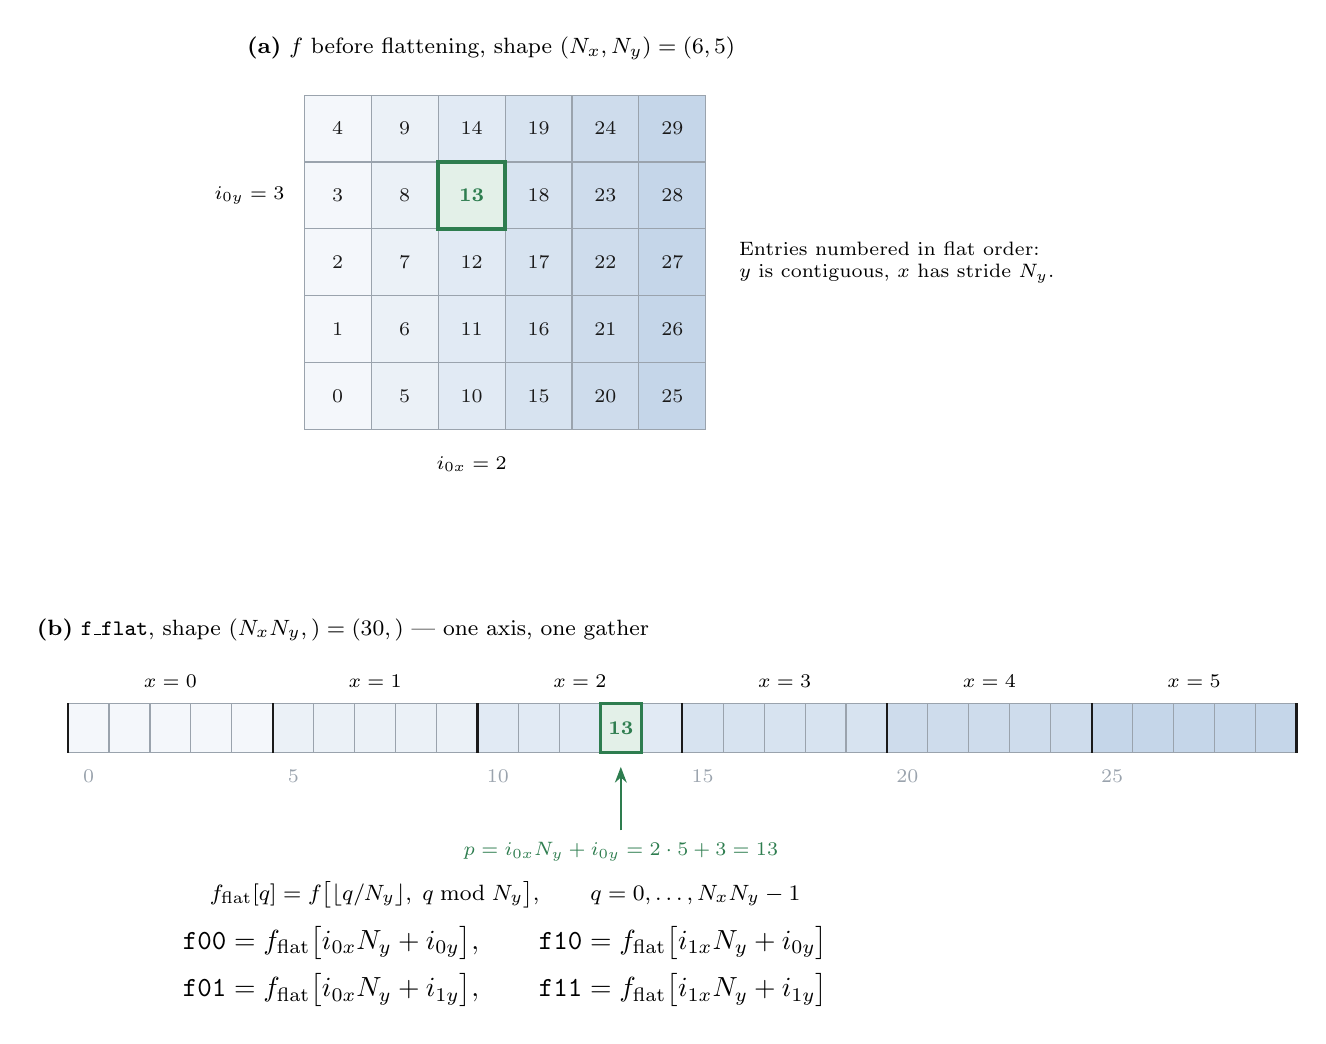
\begin{tikzpicture}[x=0.85cm,y=0.85cm]
  % ---------- 2D grid ----------
  \begin{scope}
    \node[lbl,anchor=west] at (-1.0,5.7) {\textbf{(a)} $f$ before flattening, shape $(N_x,N_y)=(6,5)$};
    \foreach \i in {0,...,5}{
      \pgfmathsetmacro{\op}{0.05+0.042*\i}
      \fill[accent,opacity=\op] (\i,0) rectangle (\i+1,5);
    }
    \draw[gridc,thin] (0,0) grid[step=1] (6,5);
    \foreach \i in {0,...,5} \foreach \j in {0,...,4} {
      \pgfmathtruncatemacro{\p}{\i*5+\j}
      \node[slbl,ink] at (\i+0.5,\j+0.5) {\p};
    }
    \fill[softg] (2,3) rectangle (3,4);
    \draw[good,very thick] (2,3) rectangle (3,4);
    \node[slbl,good] at (2.5,3.5) {\textbf{13}};
    \node[slbl,anchor=north] at (2.5,-0.25) {$i_{0x}=2$};
    \node[slbl,anchor=east] at (-0.15,3.5) {$i_{0y}=3$};
    \node[slbl,anchor=west,align=left] at (6.35,2.5)
      {Entries numbered in flat order:\\ $y$ is contiguous, $x$ has stride $N_y$.};
  \end{scope}
  % ---------- flat strip ----------
  \begin{scope}[yshift=-4.1cm,xshift=-3.0cm,x=0.52cm,y=0.52cm]
    \node[lbl,anchor=west] at (-1.0,3.0) {\textbf{(b)} \texttt{f\_flat}, shape $(N_xN_y,)=(30,)$ --- one axis, one gather};
    \foreach \p in {0,...,29}{
      \pgfmathtruncatemacro{\ii}{int(\p/5)}
      \pgfmathsetmacro{\op}{0.05+0.042*\ii}
      \fill[accent,opacity=\op] (\p,0) rectangle (\p+1,1.2);
      \draw[gridc,thin] (\p,0) rectangle (\p+1,1.2);
    }
    \foreach \p in {0,5,10,15,20,25} \draw[ink,thick] (\p,0) -- (\p,1.2);
    \draw[ink,thick] (30,0) -- (30,1.2);
    \fill[softg] (13,0) rectangle (14,1.2);
    \draw[good,very thick] (13,0) rectangle (14,1.2);
    \node[slbl,good] at (13.5,0.6) {\textbf{13}};
    \foreach \p in {0,5,10,15,20,25} \node[slbl,gridc,anchor=north] at (\p+0.5,-0.2) {\p};
    \foreach \ii in {0,...,5} \node[slbl,anchor=south] at (\ii*5+2.5,1.35) {$x=\ii$};
    \draw[good,thick,-{Stealth[length=2mm]}] (13.5,-1.9) -- (13.5,-0.35);
    \node[slbl,good,anchor=north] at (13.5,-1.95) {$p=i_{0x}N_y+i_{0y}=2\cdot 5+3=13$};
  \end{scope}
  \node[anchor=north,align=center] at (3.0,-6.6)
  {\footnotesize
   $\displaystyle f_{\rm flat}[q]=f\big[\lfloor q/N_y\rfloor,\; q\bmod N_y\big],
    \qquad q=0,\dots,N_xN_y-1$\\[6pt]
   $\displaystyle \texttt{f00}=f_{\rm flat}\big[i_{0x}N_y+i_{0y}\big],\qquad
     \texttt{f10}=f_{\rm flat}\big[i_{1x}N_y+i_{0y}\big]$\\[4pt]
   $\displaystyle \texttt{f01}=f_{\rm flat}\big[i_{0x}N_y+i_{1y}\big],\qquad
     \texttt{f11}=f_{\rm flat}\big[i_{1x}N_y+i_{1y}\big]$};

\end{tikzpicture}
\end{document}
